	\documentclass[12pt, twoside]{article}
\usepackage{jmlda}
\newcommand{\hdir}{.}
\newcommand{\mb}[1]{\mathbf{#1}}
% Здесь можно определять собственные команды, они будут действовать только внутри статьи:
\newenvironment{coderes}%
    {\medskip\tabcolsep=0pt\begin{tabular}{>{\small}l@{\quad}|@{\quad}l}}%
    {\end{tabular}\medskip}

\begin{document}

\title{Раннее прогнозирование достаточного объема выборки для обобщенно линейной модели}
\author{Жолобов В. А. Малиновский Г. Стрижов В. В.}
%\email{info@jmlda.org}
%\organization{ФИЦ <<Информатика и управление>> РАН, г.~Москва, ул.~Вавилова, 44/2}
\abstract{Исследуется проблема планирования эксперимента. Задача ранего прогнозирования важна в медицинском применении, особенно в случаях дорогостоящих измерений иммунных биомаркеров. Решается задача оценивания достаточного объема выборки для поиска адекватной регрессионной модели. Предполагается, что выборка является простой. Она описывается адеватной моделью. Иначе, выборка порождается фиксированной вероятностной моделью из известного класса моделей. Объем выборки считается достаточным, если модель восстанавливается с достаточной достоверностью. Исследуется зависимость функции ошибки от объема данных. Исследуется зависимость модели от редуцированной матрицы ковариации параметров $GLM$. Требуется, зная модель, оценить достаточный объем выборки на ранних этапах сбора данных. Предлагаются алгоритмы оценки достаточного объема выборки. Проведен вычислительный эксперимент с использованием синтетических данных.}
\titleEng{Style guide for authors}
\authorEng{JMLDA editorial board}
\organizationEng{Federal Research Center ``Computer Science and Control'' of RAS, 44/2~Vavilova~st., Moscow, Russia}
\abstractEng{
    This document explains how to prepare papers using \LaTeXe\ typesetting system and \texttt{jmlda.sty} package.
}
%\doi{10.21469/22233792}
%\receivedRus{01.01.2017}
%\receivedEng{January 01, 2017}

\maketitle
%\linenumbers
\section{Введение}
%связана с планированием эксперимента.
%Как снизить стоимость данных для исследований в несколько раз?
%Каким образом предсказать ее минимально необходимый объем по небольшому числу измерений?
%, порядка трех тысяч евро
Работа посвящена задаче оценивания достаточного объема выборки на раннем этапе сбора данных. Задача возникла из условия, когда необходимо провести крупное исследование, а сбор данных является дорогостоящим. Для примера можно взять медицинское исследование, такой как анализ крови. Существуют такие виды анализа крови, которые стоят достаточно приличных денег для людей. Для того, чтобы снизить стоимость данных для исследований в несколько раз необходимо построить модель, а для модели нужно собрать выборку. Поэтому в данной работе рассматривается задача построения алгоритма для предсказания оптимального набора данных при заданной модели. Предлагаемый в данной работе метод должен на малой выборке спрогнозировать ошибку на пополняемой большой. Выборка считается простой, то есть удовлеторяет простому распределению. Предлагается использовать два разных метода: полного перебора и генетический алгоритм.
 %При планировании эксперимента требуется оценить минимальный объем данных - количество производимых измерений некоторого набора параметров. 
  
Кроме этих методов ранее задача прогнозирования достаточного объема выборкы решалась в работе~\cite{oai:dialnet.unirioja.es:ART0000605621}. Здесь был предложен метод, основанный на технике кросс-валидации и расстоянии Кульбака-Лейблера между двумя распределениями параметров модели, оцениваемых на аналогичных подмножествах данных. Похожая задача информационного поиска решалась в работах~\cite{journals/eswa/KulunchakovS17, oai:HAL:hal-01118844v1}. Здесь для создания простых структурированных функций информационного поиска используется модернизированный генетический алгоритм. Эвристика генетического алгоритма заключается в том, что он способен работать при стагнации признаков.

В данной работе используются два метода. Основной из них~--- это метод полного перебора. Необходимо подобрать такую функцию, которая являетсямонотонной и достаточно гладкой, то есть гарантируется непрерывная дифференцируемость до второго порядка. Метод заключается в том, что он аппроксимирует зависимость функции ошибки от объема данных по малому объему выборки, чтобы с достаточной точностью предсказывать ее поведение. Считается, что модель в этой задаче задана и зависит от редуцированной матрицы ковариации параметров $GLM$. Также предложен способ генерации такой функции через генетический алгоритм.



Вычислительный эксперимент проводится на синтетических данных $Boston\ Housing$ и $Diabets$. Вначале реализуем метод полного перебора. Разделяем выборку на два множества. Строим два графика поверхности выборок: первую получаем с помощью бутстрепа~\cite{Bishop06} для подвыборки фиксированного объема, вторую через аппроксимацию. Чтобы получить аппроксимирующую поверхность, решается оптимизационную задачу. Затем повторяем действия, используя уже для поиска аппроксимирующей функции генетический алгоритм. Решение этой задачи позволит находить оптимальное значение объема выборки. 

\section{Постановка задачи}
Задана выборка $\mathfrak{D} = [\mathbf{X}, \mb{y}] = \{(\mb{x}_i, y_i)\}$, являющаяся $i.i.d.$ произвольных значений, сгенерированных неизвестным распределением. Обозначим объем выборки как $m = |\mathfrak{D}|$. Решается задача раннего прогнозирования объема минимально необходимой выборки. Под ранним прогнозированием понимается прогнозирование при однократно заданном объеме $m_0$ объема $m^*$, необходимого для построения адекватной модели. При решении задачи прогнозирования оптимального объема выборки считаем заданным модель, то есть функцию $f: \mb{x} \mapsto y$. Для отображения $f$ задаются функции ошибки, указывающая на точность модели в задачах линейной и логистической регрессиий $$S = S(\mathfrak{D}, f, w^*, m) = ||f - y||^2$$ $$S(\textbf{w}, \mathfrak{D}) = \sum_{i=1}^n\log(1 + \exp(-y_i(\textbf{w},\textbf{x}_i)))$$ Предполагается фиксированность всех параметров, кроме объема данных. Предполагается, что функция ошибки является стабилизирующей эмпирической функцией. На графике такая функция продемонстрирована. 
\begin{figure}[!htb]
\center{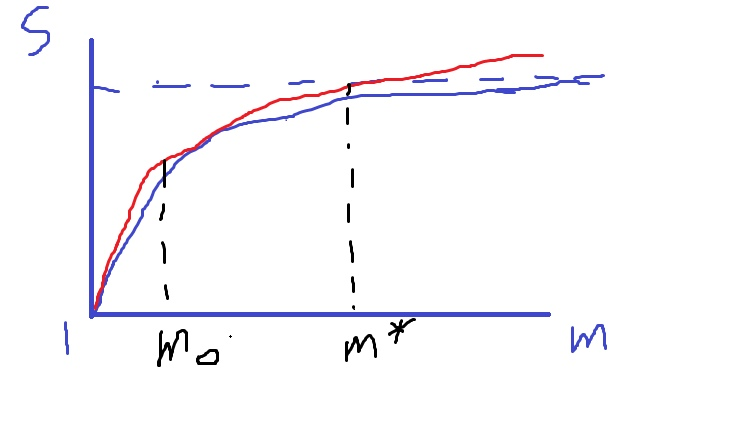
\includegraphics[width=0.6\textwidth]{scheme1}}
\end{figure}

Рассматривается несколько постановок задач обобщенной линейной модели. Первой будет задача линейной регрессии. Пусть дано множество из $m$ пар $(x_i, y_i),\ i = 1,\ldots, m$, а также пусть назначена линейная модель с аддитивной случайной величиной $\epsilon_i$ $$y_i = f(\textbf{w}, \textbf{x}_i) + \epsilon_i$$ Требуется найти параметры регрессионной модели $\textbf{w}^*$ $$\textbf{w}^* = \underset{\textbf{w} \in \mathbb{R}^n}{\text{arg} \min}S(w| \mathfrak{D}, f), $$
где $S$~--- функция ошибки.

Постановка задачи логистической регрессии. Считаем, что здесь принята модель логистической регрессии, согласно которой свободные переменные $x$ и зависимая переменная $y$ связаны зависимостью $$z = w_0 + \sum_{j=1}^nw_jx_j.$$ $$y = \frac{1}{1 + \exp(-z)} + \epsilon,$$ Обозначим $p_i = f(w, x_i)$. Функция ошибки $$S(\textbf{w}, \mathfrak{D}) = \sum_{i=1}^n\log(1 + \exp(-y_i(\textbf{w},\textbf{x}_i)))$$

В задаче поиска оптимального состава признаков $X_{\mathcal{A}}$ требуется оптимизировать набор признаков $n^* = |A|$ и $$A^* = \text{arg} \min Q(A| \textbf{w}, \mathfrak{D})$$

%При решении задачи поиска оптимального объема выборки считаем заданным модель, то есть функцию $f: \mb{x} \mapsto y$. Для отображения $f$ задается функция ошибки, указывающая на точность модели $$S = S(\mathfrak{D}, f, w^*, m) = ||f - y||^2$$ 
Обозначим зависимость значения функции ошибки от выборки как $S(m) = S(m| \textbf{w}, \mathcal{A}, \mathfrak{D})$. Так как функция $S$ зависит от объема данных, то и при каждом значении $m$ решается отдельная обобщенно-линейная задача $w^* = w^*(m)$.

%Задача раннего прогнозирования заключается в том, чтобы определить оптимальный объем данных, по которым можно построить аппроксимирующую функцию $\varphi(m)$ для функции $S(m)$. Для каждого фиксированного $m_0$ строится функция $\varphi(m)$ из оптимизационной задачи $$\varphi^*(m, m_0) = \underset{\varphi(m) \in \mathbb{C}^2(\mathbb{R}_+), \varphi'(m) \geq 0, m \in [0, m_0]}{\text{arg} \min} ||\varphi(m) - S(m)||_1$$ Затем считается ошибка аппроксимации функции ошибки $S(m)$. Искомым оптимальным объемом данных будет $$m_0^* = \underset{m_0 > 0}{\text{arg} \min}||\varphi^*(m, m_0) - S(m)||_1$$

В задаче раннего прогнозирования предполагается заданной ожидаемая точность $r$. По заданной выборке $\mathfrak{D}(m_0)$ необходимо построить функцию $\varphi(m)$, аппроксимирующую эмпирическую функцию $S(m)$. Функция $\varphi: \mathbb{N} \rightarrow \mathbb{R}_+$ выбирается из заданного класса с ограничением, связанным с принадлежностью функции $\varphi(m)$ классу дважды непрерывно дифференцируемых функций $E \subset \mathbb{C}^2(\mathbb{R}_+)$ Для поиска функции решается условная оптимизационная задача 
\begin{equation}\label{eq_app_1}
\varphi^*(m) = \underset{\varphi(m) \in E, m \in [0, m_0]}{\text{arg} \min} ||\varphi(m) - S(m)||_1
\end{equation} 
Для решения задачи выбирается функция $\varphi^*(m)$ и ищется прообраз в значении заданной точности $$m^* = (\varphi^*)^{-1}(r)$$
\section{Вычислительный эксперимент}
Эксперимент предлагается проводить в несколько этапов. На первом этапе строится линейная модель, в данном случае линейная регрессия. Полученная функция ошибки модели используется в дальнейшем. Второй этап состоит из аппроксимации функции ошибки предыдущего этапа при фиксированном числе параметров выборки на заданном семействе аппроксимирующих функций. Третий этап подразумевает аппроксимацию функции ошибки путем генетического алгоритма. На четвертом этапе решается задача с учетом решения вспомогательной задачи отбора важных признаков. На пятом этапе исследуется зависимость оптимального объема выборки от доступного размера выборки.

Для анализа алгоритма предлагается использовать три различных выборки, описания которых приведены в Таблице~\ref{table:sample}
\begin{table}[H]
\begin{center}
\caption{Описание выборок}
\begin{tabular}{|c|c|c|c|}
\hline
Выборка & Тип задачи & Размер выборки & Число признаков \\
\hline
Boston & Регрессия & $506$ & $13$ \\
\hline
Servo & Регрессия & $167$ & $4$ \\
\hline
Synthetic $1$ & Регрессия & $50000$ & $4$ \\
\hline
\end{tabular}
\label{table:sample}
\end{center}
\end{table}
Синтетическая выборка Synthetic $1$ генерирует данные из равномерного распределения на интервале $[0,1)$.
\subsection{Случай заданного семейства аппроксимирующих функций}
Для начала фиксируется выборка Boston и строится зависимость эмпирической ошибки линейной регрессии от объема выборки с учетом дисперсии. 

\begin{figure}[!htb]
\center{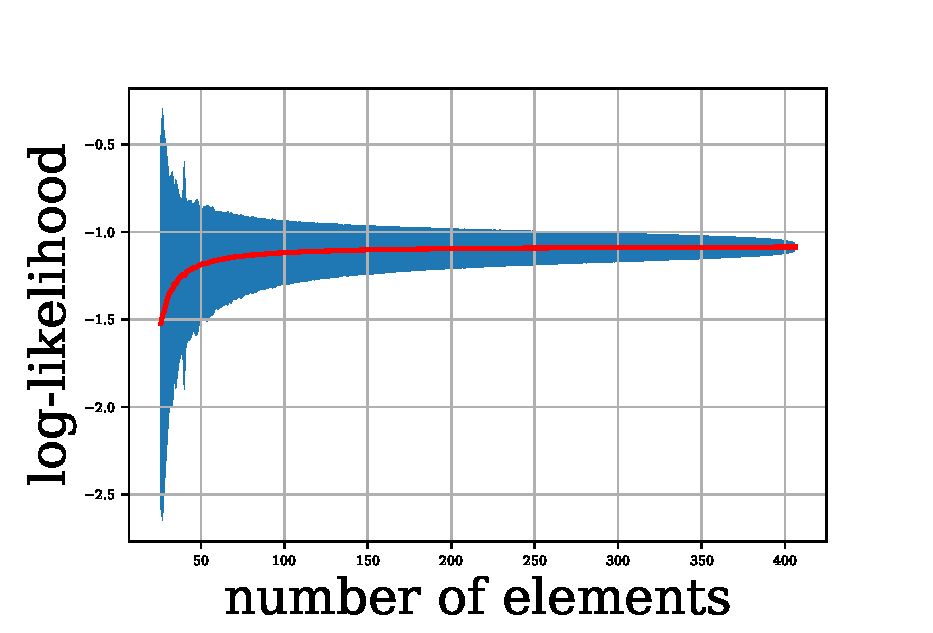
\includegraphics[width=0.6\textwidth]{BasicGraph.eps}}
\end{figure}

Видно, что гипотеза о стабилизирующейся эмпирической функции ошибки работает: подтверждается экспериментально на конкретной выборке.
Модель аппроксимирующих функций задается таким образом $$E = \{\exp(w_1 + w_2\ln m) + w_3 + w_4 \ln m | w_2 > 0\}$$ При заданном объеме выборки $m_0$ производим подбор набора коэффициентов $\textbf{w} = (w_1, w_2, w_3, w_4)$ Так ищется функция $\varphi(m)$ из задачи~\eqref{eq_app_1}
Затем по заданной точности $r$ восстанавливаем прообраз функции $\varphi(m)$. Найденное значение и есть ответ на задачу.
В случае выборки Boston построим ее поверхность 

В первом случае предполагаем число параметров фиксированным. В этом случае строим график зависимости функции ошибки от объема выборки на плоскости. Вертикальной штриховкой $---$ обозначается положение $m_0$. Есть наиболее используемый класс функций для оценки роста монотонных моделей. Если пытаться использовать каждую в отдельности, то итоговая ошибка будет слишком велика. Это видно на графике, как только объем выборки становится больше, чем $m_0$. В случае использовании их как в параметрическом семействе, то ошибка становится значительно меньше. 

\bibliographystyle{unsrt}
\bibliography{Cites}

\end{document}
